\newpage

\begin{center}
\section{Design Viewpoints}
\end{center}

\subsection{Introduction}
\qquad In this part, six main design viewpoints will be explained in detail.
\begin{itemize}
  \item Context Viewpoint
  \item Composition Viewpoint
  \item Logical Viewpoint
  \item Dependency Viewpoint
  \item Interaction Viewpoint
  \item State Dynamics Viewpoint
\end{itemize}
\qquad During this section, UML diagrams will be used to increase understandability. 

\subsection{Context Viewpoint}
\underline{\textbf{User functions:}}\\
\textbf{Register to the system:}The user will be able to register into system manually to access opportunities of the application.\\
\textbf{Login:} The user will be able to login our application after successful registration.\\
\textbf{Create event:} The user will be able to create an event.\\
\textbf{Invite users:} The user will be able to invite other users to his events.\\

\textbf{View calendars:} The user will be able to view other user’s public calendars.\\

\textbf{Answer event invitation:} The user will be able to accept or decline invitations for events.\\

\textbf{Modify calendar visibility:} The user will be able to update the visibility of his calendar to

public/private.\\

\textbf{Import/export calendar:} the user will be able to import or/and export calendars.\\

\textbf{Search user:} the user will be able to search user from users of the system.\\

\textbf{Search event:} The user will be able to search an event from all available event in the system.\\

\textbf{Modify profile:} The user will be able to update his profile data.\\

\textbf{Modify event:} The user will be able to update his events.\\

\textbf{Delate event:} The user will be able to delate any for his events.\\

\underline{\textbf{System functions:}}\\

\textbf{Notify users:} the system will notify user in case of weather forecast updates.\\

\textbf{Notify by email:} The system will notify user by email in case of weather forecast updates.\\

\textbf{Notify every 12h:} The system will notify users when they login every 12 hours in case weather

forecast updates.\\

\textbf{Notify every 3 days:} The system will notify users when they login every 3 days in case weather

forecast updates.\\

\textbf{Avoid conflicts event:} The system warn the user when he create an event in the same time as

another created event.\\
\newpage
\begin{figure}[tbh]
  \begin{center}
  % Requires \usepackage{graphicx}
  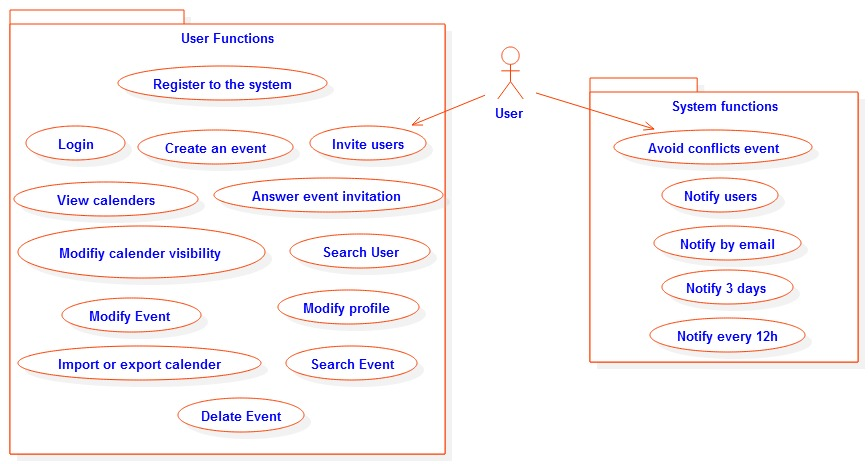
\includegraphics[width=180mm]{usecases}
    \caption{UseCases}\label{Fig 1:}
  \end{center}
\end{figure}
\newpage
\subsection{Composition Viewpoint}
\qquad Our system is composed of following components: HTML Client, HTTP Services (Servlet and JSF) EJB Container and MySQL Database. Database is placed at the lowest level of the system. HTML Client is basically the internet browser navigated to our application. Clients are connected to Enterprise Java Beans via Java Server Faces. And finally database transactions are handled by Eclipse Link framework though a JDBC connection.

\begin{figure}[tbh]
  \begin{center}
  % Requires \usepackage{graphicx}
  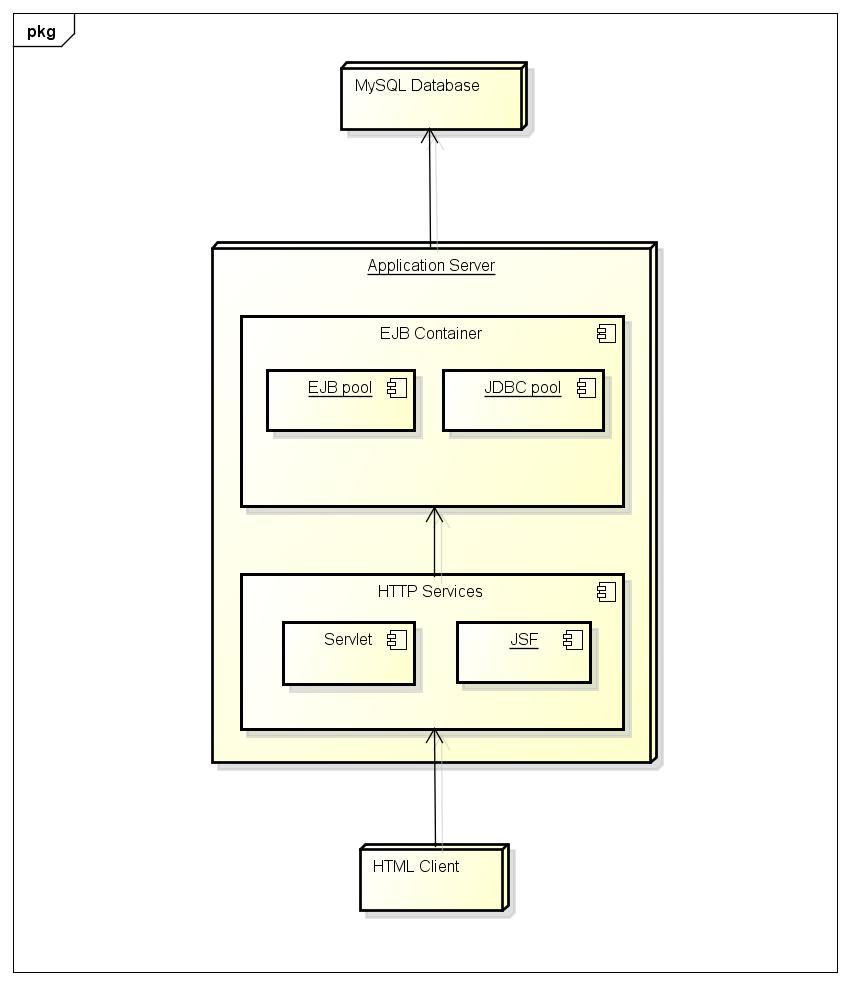
\includegraphics[width=70mm]{deployd}
    \caption{Deployment Diagram}\label{Fig 1:}
  \end{center}
\end{figure}
\qquad\textbf{MySQL Database:} Database server provides database services to clients. There are some advantages of database server, these are:
\begin{itemize}
  \setlength{\itemsep}{1pt}
    \setlength{\parskip}{1pt}
  \item	The database offers a single repository of data
  \item	Having a single stored database makes it easier to maintain the accuracy and currency of the data
  \item A single database makes it easier to protect against loss of data due to hardware failure
\end{itemize}
\qquad For database server we have selected MySQL which is an open source system and from everyone to anyone can use it. MySQL is the most opted form of database because of cross platform operability.
\par\textbf{Application Server:} As an application server, Glassfish v4.1 and JAVA EE capabilities with Enterprise Java Beans will be used.
\par EJB comes with the following advantages: "The EJB specification intends to provide a standard way to implement the back-end 'business' code typically found in enterprise applications (as opposed to 'front-end' interface code). Such code addresses the same types of problems, and solutions to these problems are often repeatedly re-implemented by programmers. Enterprise JavaBeans are intended to handle such common concerns as persistence, transactional integrity, and security in a standard way, leaving programmers free to concentrate on the particular problem at hand."
\par \textbf{Client:} The only client side in our project is HTML Client. HTML codes are generated by JSF framework included in the EJB service. In order to make User Interface development easier, PrimeFaces v5.1 library is added as a dependency to our project.
\subsection{Logical Viewpoint}
\qquad In this part of design document, the classes which we will use in our project and the relationship between classes are explained in detail. Firstly, all classes are explained with class diagram separately. After that the entity relationship diagram, which defines the database structure of our project, will be provided.
\par There are only three classes which are User, Event and weather. In the following sections, each class will be explained separately.
\begin{figure}[tbh]
  \begin{center}
  % Requires \usepackage{graphicx}
  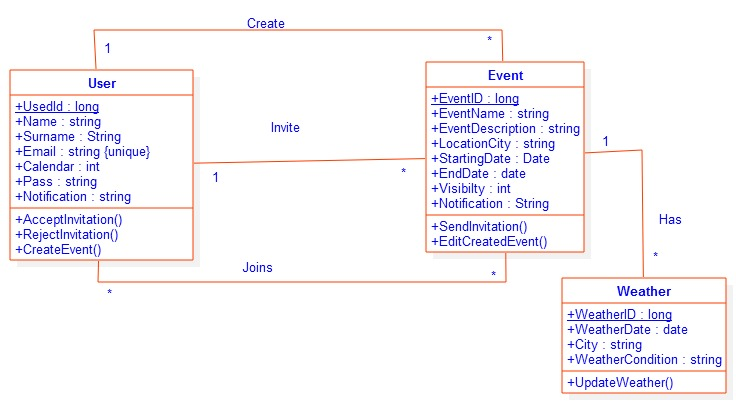
\includegraphics[width=80mm]{logical}
   % \caption{1.1)	Component Diagram}\label{Fig 1:}
  \end{center}
\end{figure}
\subsubsection{User Class}
\par User class will handle user related data operations of the system and contain all user information with invited participated and created events.
\par
\begin{figure}[tbh]
  \begin{center}
  % Requires \usepackage{graphicx}
  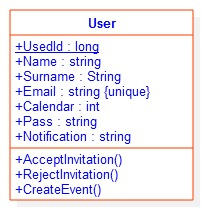
\includegraphics[width=30mm]{userclass}
   % \caption{1.1)	Component Diagram}\label{Fig 1:}
  \end{center}
\end{figure}
\begin{tabular}{|l|l|l|l|}
  \hline
  \textbf{Name} & \textbf{Type/Return Value Type} & \textbf{Visibility} & \textbf{Definition} \\
  \hline
  User\_id & Long & Private & Unique id of the user \\
  \hline
  Name & String & Private & Name of the user \\
  \hline
  Surname & String & Private & Surname of the user \\
  \hline
  Email & String & Private & Unique email address of the user \\
  \hline
  Pass & String & Private & Password of the user account \\
  \hline
  Calendar & Integer & Private & Calendar visibility of the user \\
  \hline
  Notification & String & Private & Notifications specific to this user \\
  \hline
  acceptInvitation() & Boolean & Public & Accept invitation from an event \\
  \hline
  rejectInvitaion() & Boolean & Public & Reject invitation from an event \\
  \hline
  createEvent() & Boolean & Public & Create new event \\
  \hline
\end{tabular}
\subsubsection{Event Class}
\par Event class will handle event related data operations of the system and contains information about the event, invited or participating users and owner of the event.
\begin{figure}[tbh]
  \begin{center}
  % Requires \usepackage{graphicx}
  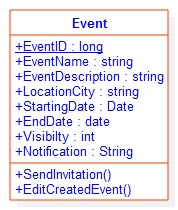
\includegraphics[width=30mm]{eventclass}
   % \caption{1.1)	Component Diagram}\label{Fig 1:}
  \end{center}
\end{figure}

\begin{tabular}{|l|l|l|l|}
  \hline
  \textbf{Name} & \textbf{Type/Return Value Type} & \textbf{Visibility} & \textbf{Definition} \\
  \hline
  Event\_id & Long & Private & Unique id of the event \\
  \hline
  Event\_name & String & Private & Name of the event \\
  \hline
  Event\_description & String & Private & Description of the event \\
  \hline
  Location\_city & String & Private & Location of the event \\
  \hline
  Starting\_date & DateTime & Private & Starting date of the event \\
  \hline
  Ending\_date & DateTime & Private & Ending date of the event \\
  \hline
  Visibility & Integer & Private & Visibility option of the event \\
  \hline
  Notification & String & Private & Notifications specific to this event \\
  \hline
  sendInvitation() & Boolean & Public & Send invitation to another \\
  & & & user from created event \\
  \hline
  editCreatedEvent() & Boolean & Public & Edit the event previously created \\
  \hline
\end{tabular}

\subsubsection{Weather Class}
\par Weather class will handle event related data operations of the system and contains information about the weather conditions in a specific location.
\begin{figure}[tbh]
  \begin{center}
  % Requires \usepackage{graphicx}
  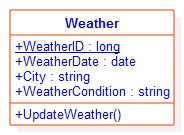
\includegraphics[width=30mm]{weather}
   % \caption{1.1)	Component Diagram}\label{Fig 1:}
  \end{center}
\end{figure}

\begin{tabular}{|l|l|l|l|}
  \hline
  \textbf{Name} & \textbf{Type/Return Value Type} & \textbf{Visibility} & \textbf{Definition} \\
  \hline
  Weather\_id & Long & Private & Unique id of the Weather \\
  \hline
  Weather\_date & Date & Private & Date of the weather forecast \\
  \hline
  City & String & Private & Location of the weather forecast \\
  \hline
  Weather\_condition & String & Private & Weather forecast \\
  \hline
  updateWeather() & Bool & Private & Updates the weather forecast \\
  \hline
\end{tabular}

\subsection{Dependency Viewpoint}
\par In this viewpoint the relationships of interconnections and access among packages are explained in detail and with UML component diagram.
\par Three-tier architecture is composed of three main packages. These are presentation tier, middle tier and data management tier.
\begin{itemize}
  \setlength{\itemsep}{1pt}
    \setlength{\parskip}{1pt}
  \item Presentation Tier: A layer that users can access directly, such as web page and client application.
  \item Middle Tier: This layer encapsulates the business such as business rules and data validation, domain concept, data access logic.
  \item Data Management Tier: The external data source to store the application data such as database server, mainframe or other legacy systems. The one we meet often today is database server.
\end{itemize}
\qquad In our system, we can divide into three basic packages. These are User Interface, Business Logic and Database. The explanation of these packages is below:
\par\textbf{User Interface:} It is top most module of our system. Basically its function is translating tasks and showing the results to the user. In User Interface package we have only one module:
\begin{itemize}
  \setlength{\itemsep}{1pt}
    \setlength{\parskip}{1pt}
  \setlength{\itemsep}{1pt}
    \setlength{\parskip}{1pt}
  \item \textbf{View:} The view can be separated into two main modules according to usage. Actually, all of these have almost same features. The View renders a presentation of modeled data. We will use HTML5 technology for client application.
\end{itemize}
\par \textbf{Business Logic:} It is the transition module of our system. The Business Logic coordinates the application, processes commands, makes logical decision and evaluation and performs calculations. It also moves and processes data between the modules, User Interface and Database in our system.
      \begin{itemize}
        \item \textbf{Model:} The model represents the part of our application that implements the business logic. It is responsible for the retrieving data and converting it into meaningful data for our application. This includes processing, validating, association or other tasks relate to handling data. We will use Java programming language for this module.
        \item \textbf{Controller:} The Controller handles requests from user. It is responsible for rendering back a response with the aid of Model module. Controller can be seen as managers taking care that all needed resources for completing a task are delegated to the correct workers. We will use Java programming language for this module.
      \end{itemize}
\qquad\textbf{Database:} It is the lowest module in our system. In this module the information is stored and retrieved from a database. The information is then passed back to the Business Logic for processing and then eventually back to the user. We will use MySQL for database package.

\begin{figure}[tbh]
  \begin{center}
  % Requires \usepackage{graphicx}
  \includegraphics[width=100mm]{compond}
    \caption{Component Diagram}\label{Fig 1:}
  \end{center}
\end{figure}

\newpage
\subsection{State Dynamics Viewpoint}
\begin{figure}[tbh]
  \begin{center}
  % Requires \usepackage{graphicx}
  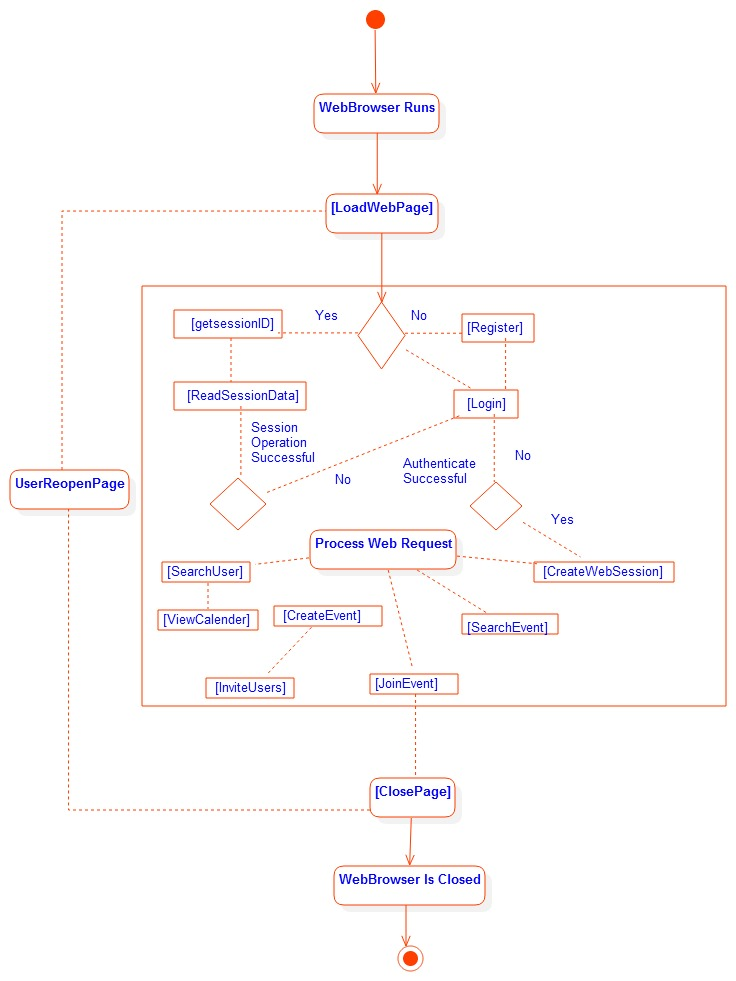
\includegraphics[width=100mm]{activity}
    \caption{Activity Diagram}\label{Fig 1:}
  \end{center}
\end{figure}

\newpage
\subsection{Interaction Viewpoint} 
\subsubsection{Register to system}
\begin{figure}[tbh]
  \begin{center}
  % Requires \usepackage{graphicx}
  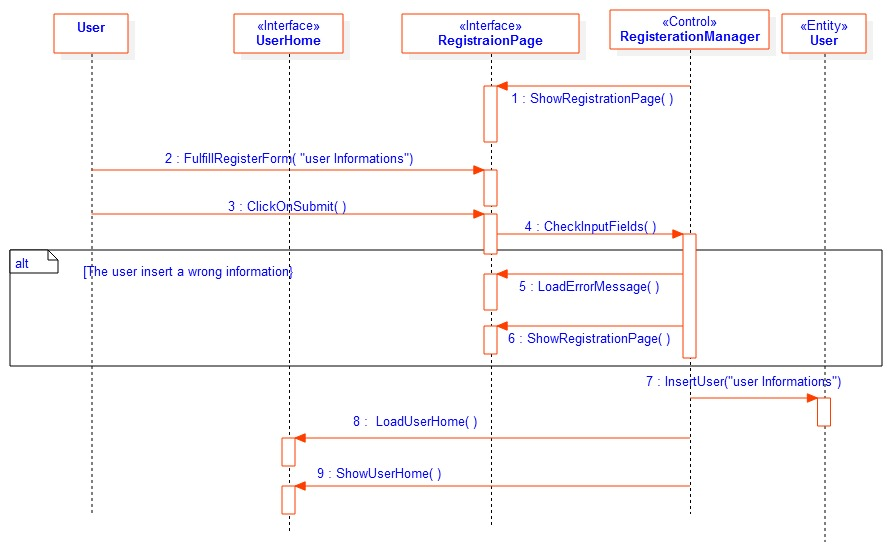
\includegraphics[width=150mm]{1reg}
    \caption{Register to system}\label{Fig 1:}
  \end{center}
\end{figure}
\newpage
\subsubsection{Modify calendar visibility}
\begin{figure}[tbh]
  \begin{center}
  % Requires \usepackage{graphicx}
  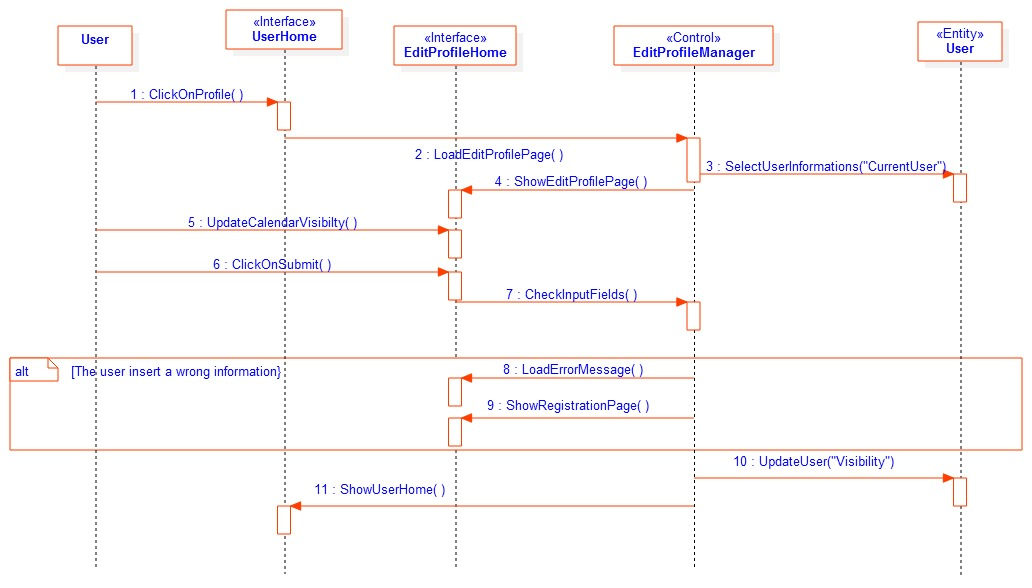
\includegraphics[width=150mm]{10modifyvisibity}
    \caption{Modify calendar visibility}\label{Fig 1:}
  \end{center}
\end{figure}
\newpage
\subsubsection{Import/Export}
\begin{figure}[tbh]
  \begin{center}
  % Requires \usepackage{graphicx}
  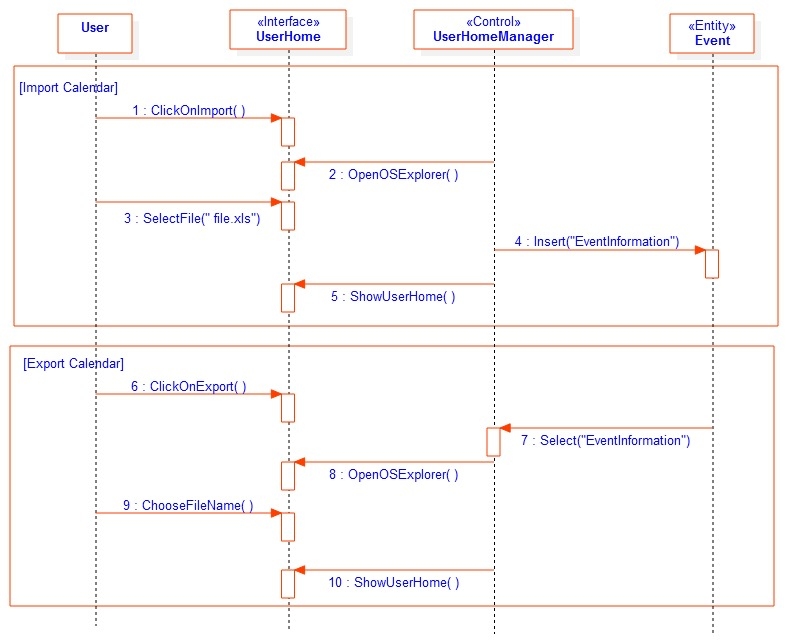
\includegraphics[width=150mm]{11import}
    \caption{Import/Export}\label{Fig 1:}
  \end{center}
\end{figure}
\newpage
\subsubsection{Search user}
\begin{figure}[tbh]
  \begin{center}
  % Requires \usepackage{graphicx}
  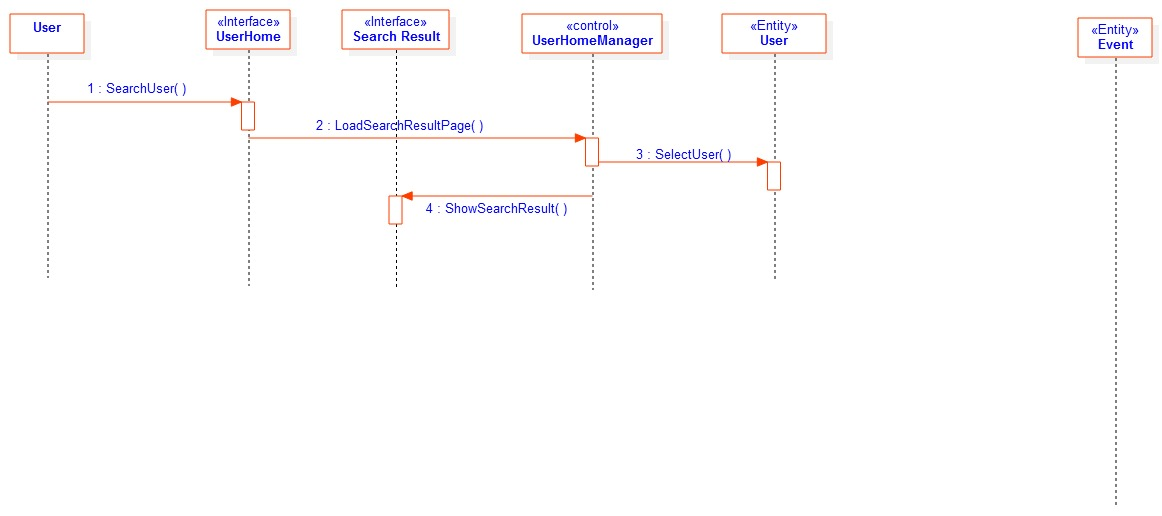
\includegraphics[width=150mm]{12search}
    \caption{Search user}\label{Fig 1:}
  \end{center}
\end{figure}

\subsubsection{Search event}
\begin{figure}[tbh]
  \begin{center}
  % Requires \usepackage{graphicx}
  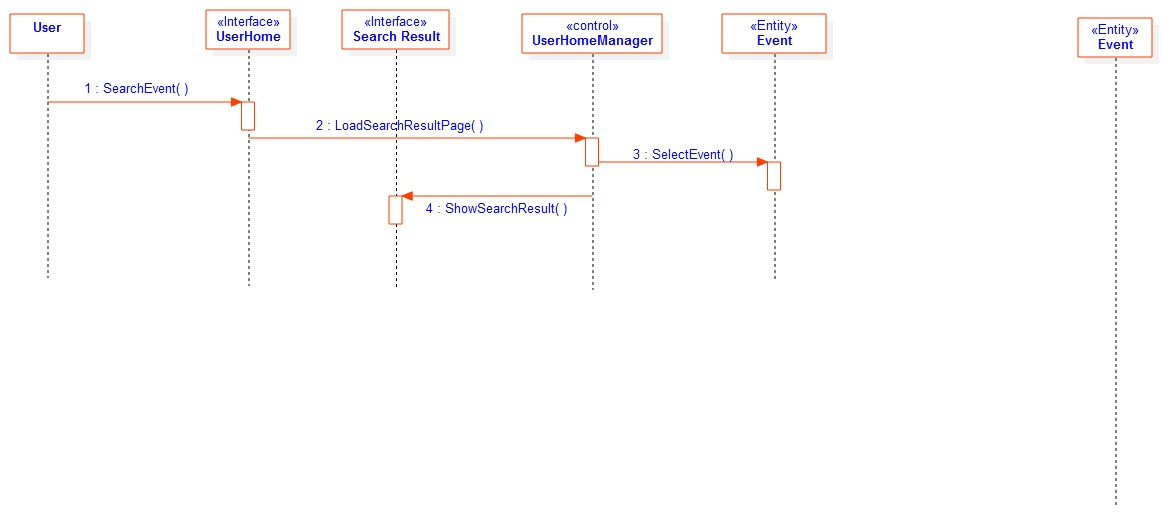
\includegraphics[width=150mm]{13search}
    \caption{Search event}\label{Fig 1:}
  \end{center}
\end{figure}
\newpage
\subsubsection{Login}
\begin{figure}[tbh]
  \begin{center}
  % Requires \usepackage{graphicx}
  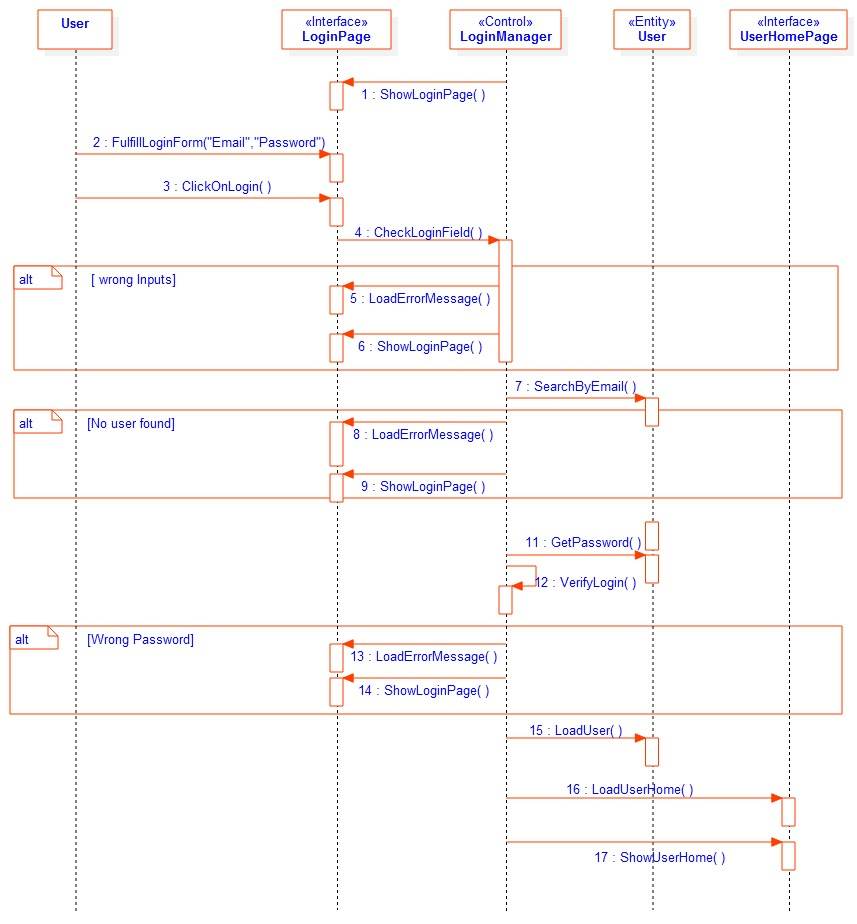
\includegraphics[width=150mm]{2log}
    \caption{Login}\label{Fig 1:}
  \end{center}
\end{figure}
\newpage
\subsubsection{Create event}
\begin{figure}[tbh]
  \begin{center}
  % Requires \usepackage{graphicx}
  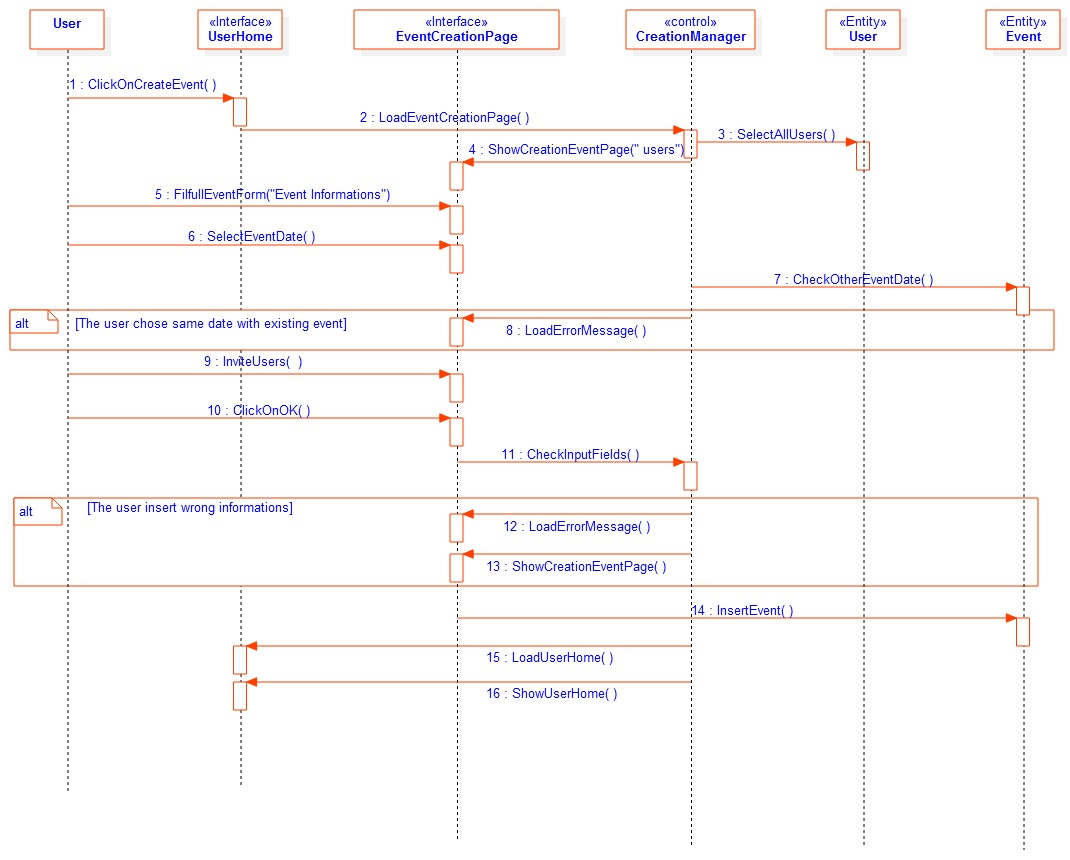
\includegraphics[width=150mm]{3create}
    \caption{Create event}\label{Fig 1:}
  \end{center}
\end{figure}
\newpage
\subsubsection{Modify event}
\begin{figure}[tbh]
  \begin{center}
  % Requires \usepackage{graphicx}
  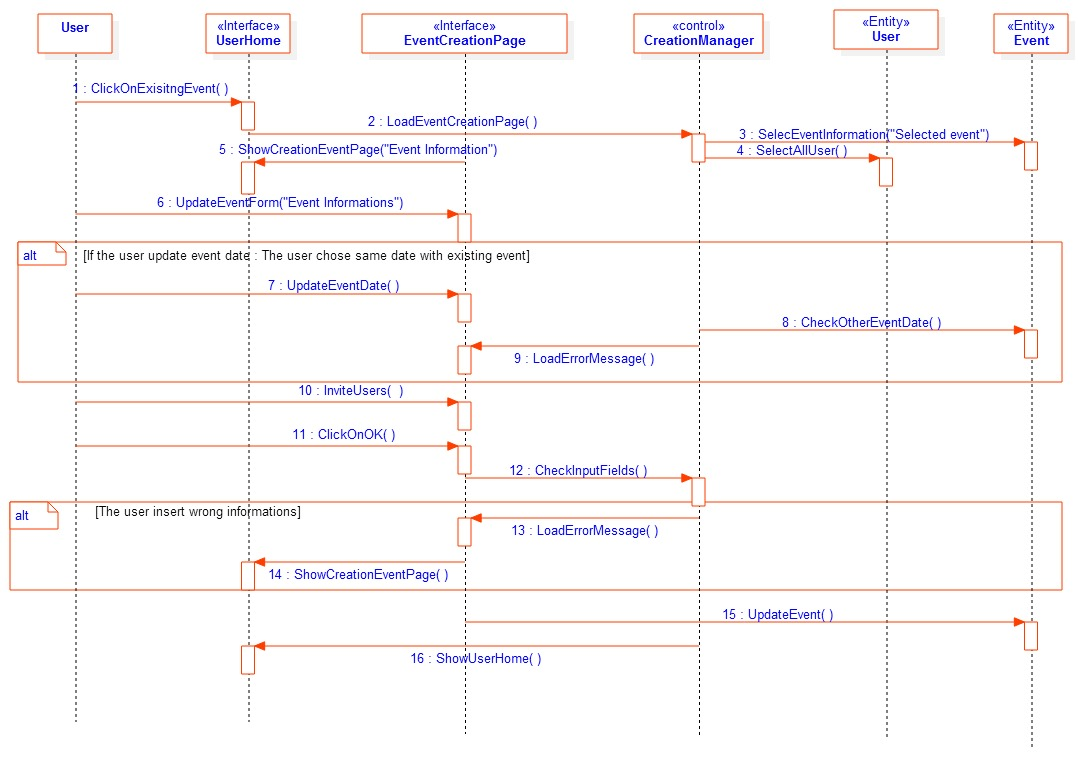
\includegraphics[width=150mm]{4modify}
    \caption{Modify event}\label{Fig 1:}
  \end{center}
\end{figure}
\newpage
\subsubsection{Delete Event}
\begin{figure}[tbh]
  \begin{center}
  % Requires \usepackage{graphicx}
  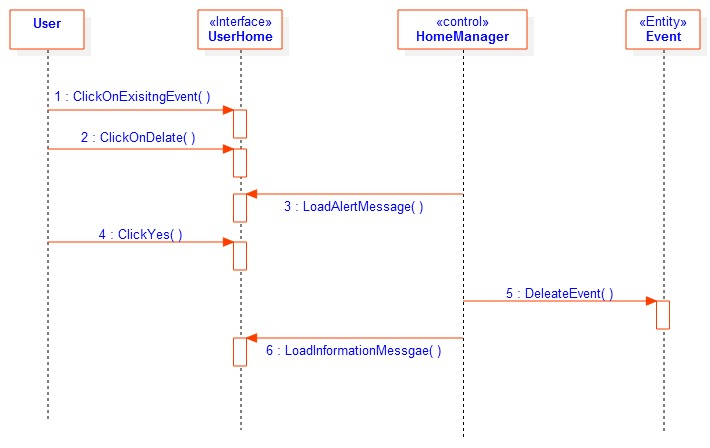
\includegraphics[width=150mm]{5delete}
    \caption{Delete Event}\label{Fig 1:}
  \end{center}
\end{figure}
\newpage
\subsubsection{Modify profile}
\begin{figure}[tbh]
  \begin{center}
  % Requires \usepackage{graphicx}
  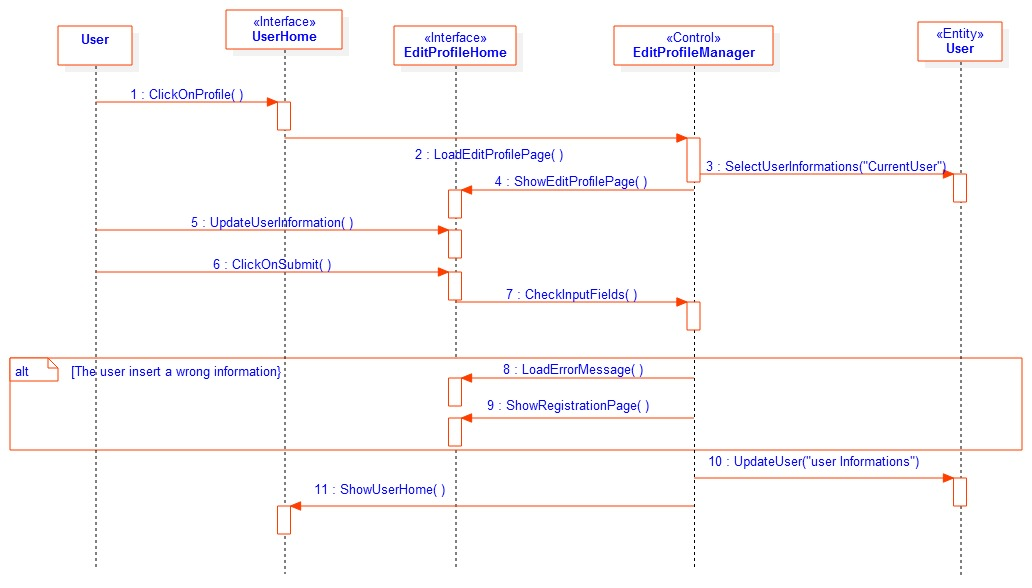
\includegraphics[width=150mm]{6modify}
    \caption{Modify profile}\label{Fig 1:}
  \end{center}
\end{figure}
\newpage
\subsubsection{Notify users}
\begin{figure}[tbh]
  \begin{center}
  % Requires \usepackage{graphicx}
  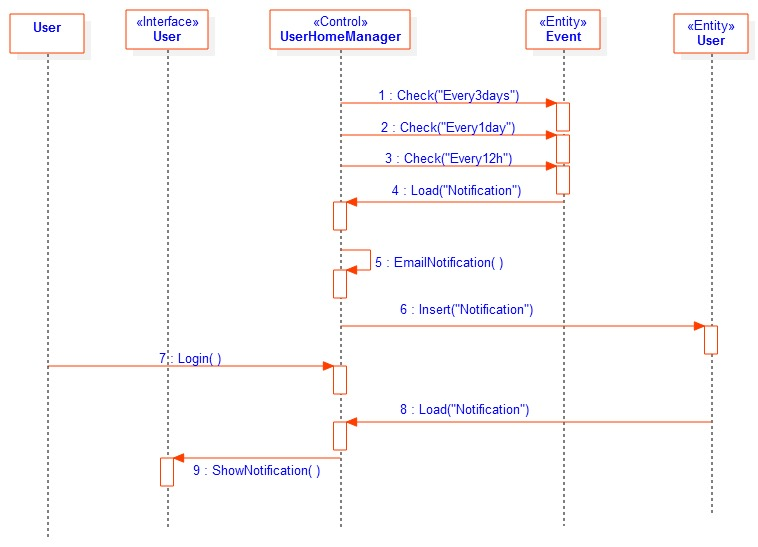
\includegraphics[width=150mm]{7notify}
    \caption{Notify users}\label{Fig 1:}
  \end{center}
\end{figure}
\newpage
\subsubsection{View calendars}
\begin{figure}[tbh]
  \begin{center}
  % Requires \usepackage{graphicx}
  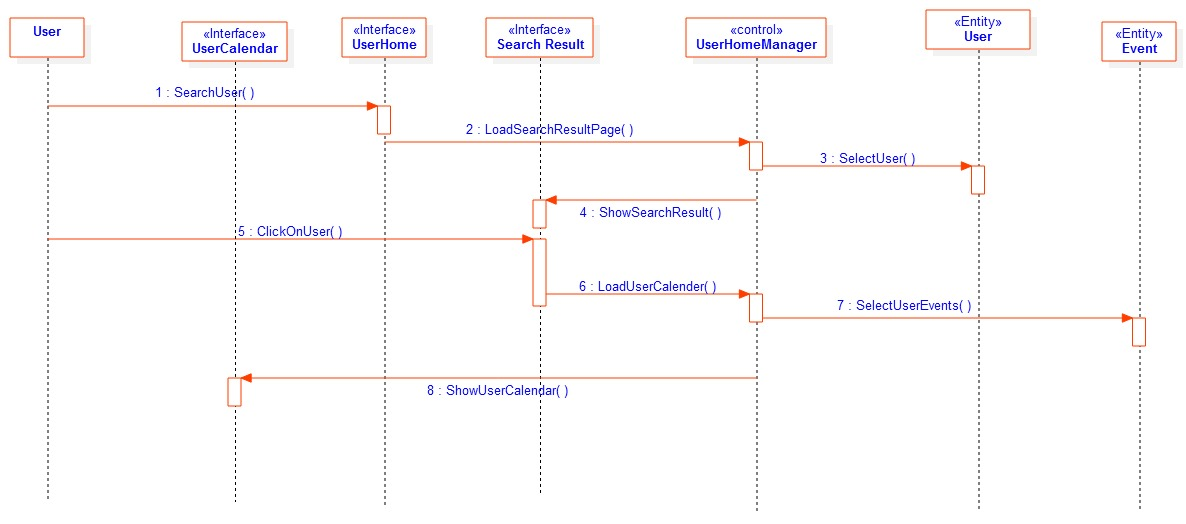
\includegraphics[width=150mm]{8view}
    \caption{View calendars}\label{Fig 1:}
  \end{center}
\end{figure}
\newpage
\subsubsection{Answer event invitation}
\begin{figure}[tbh]
  \begin{center}
  % Requires \usepackage{graphicx}
  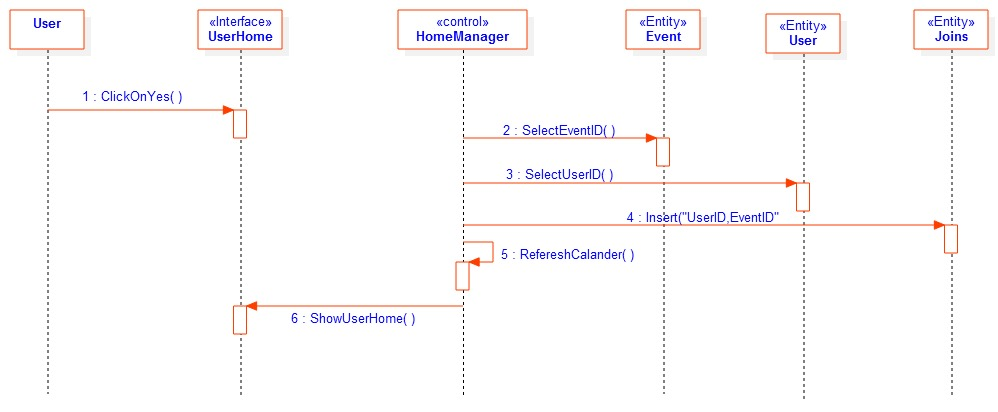
\includegraphics[width=150mm]{9answereventInvitation}
    \caption{Answer event invitation}\label{Fig 1:}
  \end{center}
\end{figure}
